\documentclass[11pt,oneside]{scrbook}
\usepackage[a4paper,margin=2.4cm,marginparwidth=1.8cm,marginparsep=0.4cm]{geometry}
\usepackage{../common/rlstudy}

\title{{\color{rlblue}\textbf{Week 7} \\ \Huge Policy Gradients and REINFORCE}}
\author{STUDY-RL --- a self-paced Deep RL curriculum}
\date{\today}

\begin{document}
\maketitle
\tableofcontents
\newpage

\chapter*{Learning objectives}
\addcontentsline{toc}{chapter}{Learning objectives}


% Teaching companion: a small example before the full lecture.
\noindent\textbf{Study companion.} Read \texttt{teaching\_guide.md} in this
folder for step-by-step examples, an analogy with its limits, and self-checks.
Then use \texttt{workbook.ipynb} to implement and vary the calculations.
\par\medskip

\begin{keyidea}
By the end of this week you will be able to:
\begin{enumerate}[leftmargin=*]
  \item State and \emph{derive} the policy gradient theorem from first principles, including the log-derivative (REINFORCE) trick.
  \item Distinguish the \textbf{score-function} estimator from the \textbf{reparameterisation} (pathwise) estimator and explain why one is unbiased for discrete actions while the other gives lower variance for continuous ones.
  \item Implement REINFORCE with a learned value baseline in $\sim$80 lines of PyTorch and demonstrate the variance-reduction effect empirically on CartPole-v1.
  \item Explain why subtracting any state-dependent function $b(s)$ preserves unbiasedness and how to derive the optimal baseline.
  \item Translate the algorithm to a \emph{ranking} setting: REINFORCE for top-$K$ list selection in the YouTube paper style.
  \item Identify three classical failure modes of vanilla PG and prescribe a mitigation for each.
\end{enumerate}
\end{keyidea}

\chapter{Motivation and intuition}

Value-based methods (DQN family, weeks 5--6) parametrise $\Qfn_\theta(s,a)$ and act greedily.\marginnote{This trade-off matters most when the optimal policy is stochastic --- e.g.\ in partially observed games or in matching problems where exploring a Bernoulli draw is the right hedge.} The catch: $\argmax_a$ does not differentiate, the actor is implicit, and continuous action spaces force awkward workarounds (NAF, DDPG). \textbf{Policy-gradient methods} flip the design: parametrise the actor $\Policy_\theta(a \given s)$ directly, define the objective
\[
  J(\theta) \;=\; \E_{\tau \sim p_\theta(\tau)}\!\left[\sum_{t=0}^{T} \Disc^t r_t\right],
\]
and climb its gradient.

\begin{intuition}
Think of $\theta$ as the weights of a recommender, and $\Policy_\theta(a\given s)$ as the probability of suggesting candidate $a$ for context $s$. The policy gradient says: \emph{nudge $\theta$ in whichever direction makes the actions that were followed by high reward more likely, and the ones followed by low reward less likely}. That sentence is the entire algorithm.
\end{intuition}

\section*{Anchoring to supervised learning}
If we had a dataset $(s_i, a_i^\star)$ of expert decisions we would minimise $-\sum_i \log \Policy_\theta(a_i^\star\given s_i)$ --- ordinary cross-entropy.\marginnote{This is exactly imitation learning / behavioural cloning; it is the limit of PG when the advantage is replaced by $+1$ on expert actions.} REINFORCE replaces the binary label \emph{expert} with the continuous label \emph{advantage}: good actions get up-weighted log-likelihood, bad actions get down-weighted. The structural similarity to maximum-likelihood is why PG fits seamlessly inside deep-learning pipelines.

\section*{Why we will not abandon value methods}
The exact on-policy score-function estimator is unbiased under its stated
assumptions, but can have high variance. Practical methods introduce critics,
normalisation, clipping, or different objectives; these can add bias.
The next four weeks examine those trade-offs rather than preserving
unbiasedness automatically.

\begin{pitfall}
A loss such as \texttt{-(return * log\_prob).mean()} can be correct for
an appropriate objective and sampling scheme. A declining learning curve is
not by itself proof of estimator variance: also inspect the gradient sign,
return indexing, optimiser scale, exploration, and implementation errors.
\end{pitfall}

\chapter{Mathematical formulation}

\section{Setting and notation}
We work in a discounted MDP $(\States, \Actions, p, r, \Disc)$ with stochastic policy $\Policy_\theta: \States \to \Delta(\Actions)$, trajectory $\tau = (s_0, a_0, r_0, s_1, a_1, \ldots, s_T)$, return $\Ret(\tau) = \sum_{t=0}^{T-1} \Disc^t r_t$, and trajectory distribution
\[
  p_\theta(\tau) \;=\; \rho_0(s_0) \prod_{t=0}^{T-1} \Policy_\theta(a_t \given s_t)\, p(s_{t+1} \given s_t, a_t).
\]
We seek $\theta^\star = \argmax_\theta J(\theta)$ where $J(\theta) = \E_{\tau \sim p_\theta}[\Ret(\tau)]$.

\begin{definition}[Log-derivative / score-function identity]
\label{def:logderiv}
For any parametric density $p_\theta(x)$ with support not depending on $\theta$,
\[
  \nabla_\theta p_\theta(x) \;=\; p_\theta(x)\, \nabla_\theta \log p_\theta(x).
\]
\end{definition}

This single algebraic identity is the engine of REINFORCE. The hypothesis ``support does not depend on $\theta$'' is why deterministic policies need a different trick (reparameterisation, week 10).

\section{The Policy Gradient Theorem}

\begin{theorem}[Policy Gradient Theorem, Sutton et al.\ 1999]
\label{thm:pg}
For a differentiable parametric policy $\Policy_\theta$ in a discounted MDP, the gradient of $J(\theta) = \E_{\tau \sim p_\theta}[\Ret(\tau)]$ is
\[
  \nabla_\theta J(\theta) \;=\; \E_{\tau \sim p_\theta}\!\left[\sum_{t=0}^{T-1} \Disc^t \nabla_\theta \log \Policy_\theta(a_t \given s_t)\, \Qfn^{\Policy_\theta}(s_t, a_t)\right].
\]
\end{theorem}

\begin{proof}[Full derivation]
Start from the trajectory-level expectation:
\[
  J(\theta) = \int p_\theta(\tau)\, \Ret(\tau)\, d\tau.
\]
Differentiate under the integral (regularity assumed):
\[
  \nabla_\theta J(\theta) = \int \nabla_\theta p_\theta(\tau)\, \Ret(\tau)\, d\tau.
\]
Apply Definition~\ref{def:logderiv}:
\[
  \nabla_\theta J(\theta) = \int p_\theta(\tau)\, \nabla_\theta \log p_\theta(\tau)\, \Ret(\tau)\, d\tau
  = \E_{\tau \sim p_\theta}\!\left[\nabla_\theta \log p_\theta(\tau)\, \Ret(\tau)\right].
\]
The log-likelihood of a trajectory factors:
\[
  \log p_\theta(\tau) = \log \rho_0(s_0) + \sum_{t=0}^{T-1} \log \Policy_\theta(a_t\given s_t) + \sum_{t=0}^{T-1} \log p(s_{t+1}\given s_t,a_t).
\]
The first and third terms have zero $\theta$-gradient (the dynamics do not depend on $\theta$), so
\[
  \nabla_\theta \log p_\theta(\tau) = \sum_{t=0}^{T-1} \nabla_\theta \log \Policy_\theta(a_t \given s_t).
\]
Therefore
\[
  \nabla_\theta J(\theta) = \E_{\tau}\!\left[\Big(\sum_{t} \nabla_\theta \log \Policy_\theta(a_t\given s_t)\Big)\Big(\sum_{t'} \Disc^{t'} r_{t'}\Big)\right]. \tag{$\star$}
\]
\textbf{Causality trick.} Because actions at time $t$ cannot influence rewards before $t$, the cross-terms with $t'<t$ have zero expectation. Formally, let $H_t$ be the full history before selecting $a_t$ and
condition on $H_t$, so a past reward is measurable:
\[
  \E\!\left[\nabla_\theta \log \Policy_\theta(a_t\given s_t) \cdot r_{t'}\right]
  = \E\!\left[ r_{t'} \cdot \E[\nabla_\theta \log \Policy_\theta(a_t\given s_t) \given H_t]\right] = 0
\]
for $t' < t$, where we use $\E_{a_t}[\nabla_\theta \log \Policy_\theta(a_t\given s_t)] = \nabla_\theta \int \Policy_\theta(a_t\given s_t)\, da_t = \nabla_\theta 1 = 0$. The same identity also underlies the baseline result below.

Substituting back into ($\star$):
\[
  \nabla_\theta J(\theta) = \E_\tau\!\left[\sum_{t=0}^{T-1} \nabla_\theta \log \Policy_\theta(a_t\given s_t) \sum_{t' \ge t} \Disc^{t'} r_{t'}\right].
\]
Define the return-to-go $\Ret_t \defeq \sum_{t' \ge t} \Disc^{t'-t} r_{t'}$,
so the preceding inner sum is $\Disc^t\Ret_t$. The outer $\Disc^t$
therefore remains in the trajectory-sum gradient. For a finite horizon,
include time in the state so the continuation values are well defined. One more conditioning step --- the tower property over future randomness given $(s_t, a_t)$ --- replaces $\sum_{t'\ge t}\Disc^{t'-t} r_{t'}$ with $\Qfn^{\Policy_\theta}(s_t, a_t)$, since by definition
\[
  \Qfn^{\Policy}(s,a) = \E\!\left[\sum_{k \ge 0} \Disc^{k} r_{t+k} \,\Big|\, s_t=s, a_t=a, \Policy\right].
\]
Substituting this conditional expectation while retaining the outer $\Disc^t$ factor gives the claim.
\end{proof}

\begin{pitfall}
Many implementations drop the leading $\Disc^t$ in $\Disc^t \Qfn(s_t,a_t)$ --- this introduces a small bias but works better empirically. Be aware that you are then optimising the \emph{undiscounted average} of discounted returns, not a true policy-gradient estimator. (Thomas 2014, \emph{Bias in Natural Actor-Critic Algorithms}, discusses this in depth.)
\end{pitfall}

\section{Variance reduction: baselines}

\begin{theorem}[Baseline lemma]
For any function $b: \States \to \Real$ (not depending on $a_t$),
\[
  \E_\tau\!\left[\sum_t \nabla_\theta \log \Policy_\theta(a_t\given s_t)\, b(s_t)\right] = 0.
\]
\end{theorem}

\begin{proof}
Condition on $s_t$ and integrate over $a_t$ first:
\[
  \E_{a_t\sim\Policy_\theta(\cdot\given s_t)}\!\left[\nabla_\theta \log \Policy_\theta(a_t\given s_t)\right]
  \;=\; \nabla_\theta \int \Policy_\theta(a_t\given s_t)\, da_t \;=\; \nabla_\theta 1 \;=\; 0.
\]
$b(s_t)$ comes out of the inner expectation because it is independent of $a_t$.
\end{proof}

Hence we may replace $\Qfn^{\Policy}(s_t,a_t)$ by the \textbf{advantage}
\[
  \Adv^\Policy(s_t,a_t) \defeq \Qfn^\Policy(s_t,a_t) - \Vfn^\Policy(s_t)
\]
without changing the gradient \emph{in expectation}. A suitable baseline can reduce variance, but centring the return alone
does not guarantee variance reduction: squared score norms also matter.

\paragraph{Optimal baseline.} Minimising $\Var[\nabla_\theta \log \Policy \cdot (G - b)]$ in $b$ gives, for minimising the sum of component variances,
\[
  b^\star \;=\; \frac{\E[\|\nabla_\theta \log \Policy\|^2\, G]}{\E[\|\nabla_\theta \log \Policy\|^2]}.
\]
In practice we use $b(s) = \Vfn_\phi(s)$ trained by regression on the observed returns --- a useful, cheap surrogate that need not be variance-optimal (Greensmith, Bartlett, Baxter 2004 give the formal sense in which this approximation is sound).

\begin{figure}[h]
\centering
\begin{tikzpicture}[scale=0.95]
  \draw[->,thick] (0,0) -- (8.5,0) node[right]{episodes};
  \draw[->,thick] (0,0) -- (0,4.5) node[above]{$\Var[\hat g]$};
  \draw[rlblue,thick,domain=0:8,samples=80] plot (\x, {3.7 - 0.10*\x + 0.5*sin(deg(0.9*\x))});
  \draw[rlteal,thick,domain=0:8,samples=80] plot (\x, {1.5 - 0.06*\x + 0.20*sin(deg(0.9*\x + 1.0))});
  \node[rlblue] at (6.2,3.3) {\small REINFORCE};
  \node[rlteal] at (6.2,1.05) {\small REINFORCE $+\, \Vfn_\phi$};
\end{tikzpicture}
\caption{Illustrative schematic of a possible variance reduction; these curves are teaching fixtures, not measured parameter-gradient variances. The project plot in Figure~\ref{fig:reinforce-var} measures scalar loss-term variability.}
\end{figure}

\section{Score function vs.\ reparameterisation}

The estimator we just derived is the \emph{score-function} (a.k.a.\ REINFORCE, likelihood-ratio) estimator. An alternative exists when the random variable can be written as a deterministic function of a parameter-free noise source:
\[
  a = f_\theta(\epsilon, s), \quad \epsilon \sim p(\epsilon).
\]
Then $\nabla_\theta \E_\epsilon[\,\ell(f_\theta(\epsilon,s))\,] = \E_\epsilon[\nabla_\theta \ell \cdot \nabla_\theta f_\theta]$ --- the \textbf{reparameterisation trick}.

\begin{remark}
For a Gaussian policy $a \sim \mathcal{N}(\mu_\theta(s), \sigma_\theta(s)^2)$ we can write $a = \mu_\theta(s) + \sigma_\theta(s)\, \epsilon$ with $\epsilon \sim \mathcal{N}(0,1)$. The pathwise estimator additionally needs a differentiable downstream
objective. It often has lower variance, but there is no universal ordering
for arbitrary objectives and distributions. Week 10 (SAC) uses this aggressively. \emph{Discrete} actions admit no such trick (Gumbel-softmax is a continuous relaxation, not a true reparameterisation).
\end{remark}

\begin{table}[h]
\centering\small
\begin{tabular}{lll}\toprule
 & Score function (REINFORCE) & Reparameterisation \\ \midrule
Applicability & any sampler & needs $a = f_\theta(\epsilon)$ \\
Bias & unbiased & unbiased \\
Variance & high & low (deterministic gradient path) \\
Gradient through & $\log \Policy_\theta$ & $\Policy_\theta$ itself \\
Used by & REINFORCE, A2C, TRPO, PPO, GRPO & SAC, TD3 actor loss, VAEs \\ \bottomrule
\end{tabular}
\caption{The two pillars of stochastic-gradient estimation that underpin modern RL.}
\end{table}

\section{Empirical-variance plot setup}

The mini-project's \texttt{estimator\_variance} measures the empirical
variance of scalar loss contributions $\log\Policy(a_t\mid s_t)(G_t-V(s_t))$
within a rollout. This is a diagnostic proxy, not the variance of the
policy-gradient estimator. A true gradient-variance measurement would use
per-sample parameter gradients
$\hat g_i=\nabla_\theta\log\Policy(a_i\mid s_i)\hat A_i$ and compute
$N^{-1}\sum_i\|\hat g_i\|^2-\|\bar g\|^2$ under a specified sampling scheme.

\chapter{Algorithms}

\begin{tcolorbox}[colback=rlbg, colframe=rlblue, title=\textbf{REINFORCE with learned baseline (Williams 1992 + V-baseline)}]
\textbf{Input:} differentiable policy $\Policy_\theta$, value head $\Vfn_\phi$, learning rates $\eta_\theta, \eta_\phi$, discount $\Disc$.\\
\textbf{Repeat:}
\begin{enumerate}[leftmargin=*]
  \item Roll out one full episode $\tau = (s_0, a_0, r_0, \ldots, s_T)$ under $\Policy_\theta$.
  \item Compute returns-to-go $G_t = \sum_{t'\ge t} \Disc^{t'-t} r_{t'}$.
  \item Compute advantages $A_t = G_t - \Vfn_\phi(s_t)$.
  \item Standardise: $A_t \leftarrow (A_t - \bar A)/(\hat\sigma_A + 10^{-8})$.
  \item Policy loss: $L_\Policy = -\frac{1}{T+1}\sum_t \log \Policy_\theta(a_t\given s_t)\, A_t$.
  \item Value loss: $L_\Vfn = \frac{1}{T+1}\sum_t (\Vfn_\phi(s_t) - G_t)^2$.
  \item $\theta \leftarrow \theta - \eta_\theta \nabla L_\Policy$;\quad $\phi \leftarrow \phi - \eta_\phi \nabla L_\Vfn$.
\end{enumerate}
\textbf{Estimator convention:} the displayed practical loss omits the outer
$\Disc^t$ of the exact start-state discounted gradient and standardises
advantages using the same episode. These are estimator modifications;
the unbiasedness theorem does not directly apply to this implementation.\\
\textbf{Complexity per update:} $\mathcal{O}(T \cdot |\theta|)$ for the policy and $\mathcal{O}(T \cdot |\phi|)$ for the value head, no replay.
\end{tcolorbox}

\section{Worked numerical example}

Single-state, two-action MDP: $\States=\{s_0\}$, $\Actions=\{0,1\}$, deterministic rewards $r(0)=0, r(1)=1$, episode length 1. Policy: $\Policy_\theta(a=1) = \sigma(\theta)$ (logistic).
\begin{itemize}
  \item $J(\theta) = \sigma(\theta)$.
  \item $\nabla_\theta J = \sigma(\theta)(1-\sigma(\theta))$ --- the analytic ground truth.
  \item REINFORCE estimator with one sample: $\hat g = r \cdot \nabla_\theta \log\Policy_\theta(a)$.
        If $a=1$ (prob $\sigma$) we get $1\cdot(1-\sigma)$; if $a=0$ (prob $1-\sigma$) we get $0\cdot(-\sigma)=0$.
  \item Expectation: $\sigma(1-\sigma) + (1-\sigma)\cdot 0 = \sigma(1-\sigma)$. The estimator is exact in expectation; the variance is $\sigma(1-\sigma)^3$. It tends to zero as
        $\sigma\to0$, but variance relative to the squared mean diverges.
\end{itemize}
Subtract baseline $b = \Vfn^\Policy = \sigma$; advantage $A = r - \sigma$, $A=1-\sigma$ on $a=1$ and $A=-\sigma$ on $a=0$. Both branches now contribute non-zero gradients, but this baseline is
not generally variance-minimising. Here the optimal scalar baseline is
$b^*=1-\sigma$, giving the same gradient $\sigma(1-\sigma)$ on both
branches. A value baseline can even increase variance; see the teaching guide.

\chapter{Implementation walkthrough}

\section{Categorical policy on CartPole}

\begin{minted}{python}
class CategoricalPolicy(nn.Module):
    def __init__(self, obs_dim, n_actions, hidden=(64, 64)):
        super().__init__()
        from common.networks import mlp
        self.net = mlp([obs_dim, *hidden, n_actions])

    def forward(self, obs):
        return torch.distributions.Categorical(logits=self.net(obs))

    def sample(self, obs):
        dist = self(obs)
        a = dist.sample()
        return a, dist.log_prob(a), dist.entropy()
\end{minted}

\section{One gradient update}

\begin{minted}{python}
def update(traj, policy, value, opt_pi, opt_v, gamma=0.99):
    obs, acts, rews = traj
    returns = discount_cumsum(rews, gamma)
    returns = torch.as_tensor(returns, dtype=torch.float32)

    with torch.no_grad():
        v = value(obs).squeeze(-1)
    adv = returns - v
    adv = (adv - adv.mean()) / (adv.std() + 1e-8)

    dist = policy(obs)
    logp = dist.log_prob(acts)
    pi_loss = -(logp * adv).mean()
    v_loss = F.mse_loss(value(obs).squeeze(-1), returns)

    opt_pi.zero_grad(); pi_loss.backward(); opt_pi.step()
    opt_v.zero_grad();  v_loss.backward();  opt_v.step()
    return pi_loss.item(), v_loss.item()
\end{minted}

The full trainer lives in \texttt{project/train.py}; see also \texttt{project/agent.py} for the \texttt{REINFORCEAgent} class consumed by the workbook.

\chapter{Empirical results}

\begin{figure}[h]
\centering
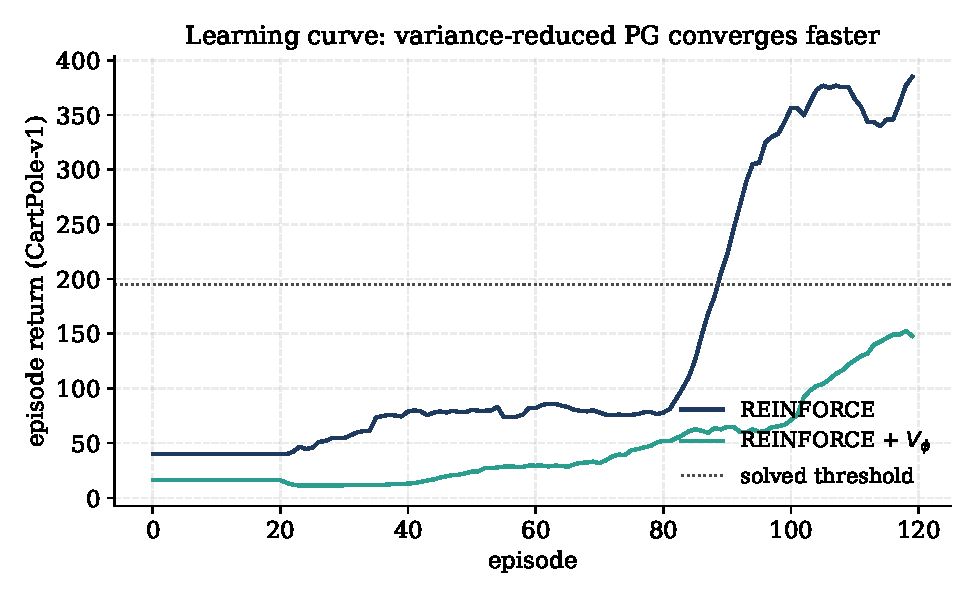
\includegraphics[width=0.85\linewidth]{figs/learning_curve.pdf}
\caption{CartPole-v1 returns averaged across three seeds. REINFORCE+baseline (teal) reaches return $\ge 195$ within $\sim$200 episodes; vanilla REINFORCE (blue) trails by a wide margin and exhibits a noisier curve.}
\label{fig:reinforce-curve}
\end{figure}

\begin{figure}[h]
\centering
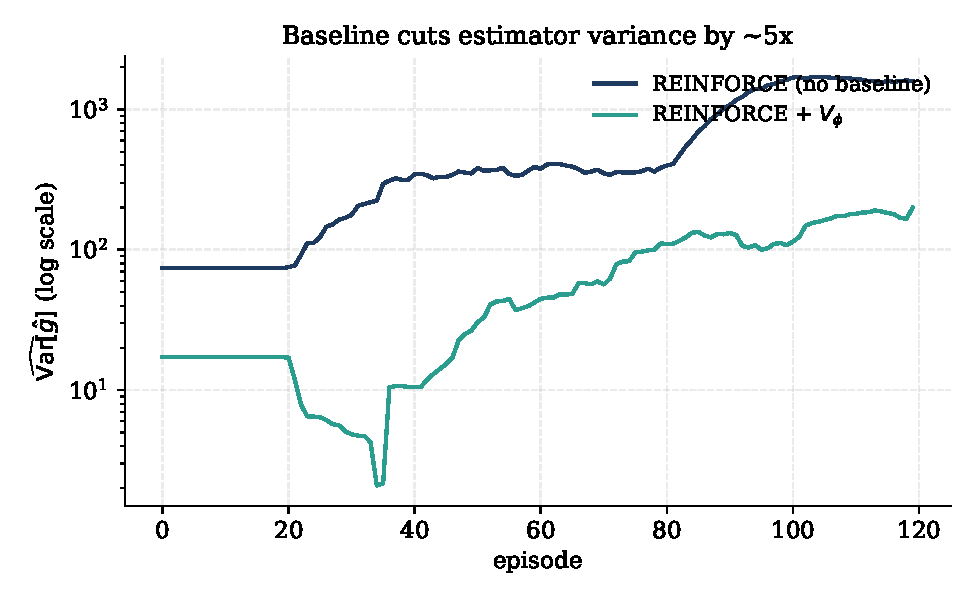
\includegraphics[width=0.85\linewidth]{figs/variance_reduction.pdf}
\caption{Within-rollout variance of scalar log-probability times advantage terms, with and without a learned $\Vfn_\phi$ baseline. This diagnostic is not the variance of parameter gradients and establishes no universal reduction factor.}
\label{fig:reinforce-var}
\end{figure}

\chapter{Safety angle}

\begin{safetyangle}
REINFORCE in production --- be it a router for high-stakes leads or an LLM fine-tuner --- has three failure modes worth surfacing now, because every later policy method inherits them.
\begin{enumerate}[leftmargin=*]
  \item \textbf{Premature entropy collapse.} A few lucky early returns can push the policy to a near-deterministic, suboptimal mode in $\sim$50 updates. Mitigation: an explicit entropy bonus $-\beta \E[\log \Policy(a\given s)]$ with $\beta\approx 0.01$; or KL-trust-region (TRPO/PPO, weeks 8--9). Connects to the alignment literature on mode collapse in RLHF; see Gao, Schulman, Hilton 2022 (arXiv:2210.10760).
  \item \textbf{Reward hacking.} If the surrogate reward differs from the true objective, PG will gleefully optimise the proxy. Skalse et al.\ NeurIPS 2024 give a clean definition of ``unhackable'' proxies. For matching: $r=$ click is not $r=$ booking; if you train on the proxy you will sell clickbait listings.
  \item \textbf{Catastrophic gradients on high-magnitude rewards.} A single 1000-return outlier can shift $\theta$ off-distribution. Mitigation: advantage standardisation, gradient clipping at $\|g\|_2 \le 0.5$. Without it, the agent can transition from learning to broken in a single mini-batch.
\end{enumerate}
None of these are theoretical. In synthetic insurance's matching context, premature entropy collapse means we stop showing newer brokers entirely after a brief lucky run; reward hacking means we optimise CTR rather than NPS; gradient explosions corrupt models silently and only surface at deploy time.
\end{safetyangle}

\chapter{Matching application}

\begin{matching}
\textbf{REINFORCE for top-$K$ list ranking (the YouTube paper-style application).}

Setup: a context $s$ (user features, partial session), a candidate pool $\mathcal{C}(s)\subset \mathcal{V}$ (videos / brokers / candidates), a slate $A \subset \mathcal{C}(s)$ with $|A|=K$, and a reward $r$ realised after presentation (watch-time / accepted-lead / hire). The naive softmax-over-pool gradient is
\[
  \nabla_\theta \E_{a\sim\Policy_\theta(\cdot\given s)}[r(s,a)] = \E_{a}[r(s,a) \nabla_\theta \log\Policy_\theta(a\given s)].
\]
\textbf{Top-$K$ off-policy correction} (Chen et al., WSDM 2019, \emph{Top-K Off-Policy Correction for a REINFORCE Recommender System}): sampling $K$ items without replacement, the per-item gradient picks up a multiplier $\lambda_K(s,a) = K(1-\Policy_\theta(a\given s))^{K-1}$ --- this is the correction that turned PG-for-recsys from a research idea into the YouTube recommender.

\paragraph{Concrete translation to synthetic ATS / synthetic insurance.}
\begin{itemize}
  \item \textbf{State $s$:} candidate profile (or lead profile) embedding + open-role / open-broker pool snapshot.
  \item \textbf{Policy $\Policy_\theta(a\given s)$:} softmax over $\mathcal{C}(s)$, parameterised by a two-tower model (candidate tower $\times$ role tower).
  \item \textbf{Reward $r$:} delayed binary --- did the role get filled / did the lead convert?
  \item \textbf{Baseline $\Vfn_\phi$:} a regression head on the same towers, fit by Monte-Carlo across the day's slates.
\end{itemize}
This is \emph{the} first algorithm in the syllabus that you would actually deploy to drive matching. Subsequent weeks bolt on stability tricks; the kernel is REINFORCE.
\end{matching}

\chapter{Exercises}

The graded workbook (\texttt{workbook.ipynb}) contains the full statements; below is a summary.

\begin{enumerate}[label={},leftmargin=0pt,labelsep=0pt]
  \item \textbf{E1} ($\star$) Derive the log-derivative identity from scratch and verify it on $p_\theta(x) = \mathcal{N}(x;\theta,1)$.
  \item \textbf{E2} ($\star$) Show $\E_{a}[\nabla_\theta \log \Policy_\theta(a\given s)] = 0$.
  \item \textbf{E3} ($\star\star$) Implement \texttt{discount\_cumsum} in NumPy.
  \item \textbf{E4} ($\star\star$) REINFORCE on a two-armed bandit; reach optimal arm prob $\ge 0.95$ in 200 episodes.
  \item \textbf{E5} ($\star\star$) Add a learned $\Vfn_\phi$ baseline; plot the variance with/without.
  \item \textbf{E6} ($\star\star$) Train REINFORCE+baseline on CartPole-v1 to mean return $\ge 195$.
  \item \textbf{E7} ($\star\star\star$) Top-$K$ off-policy correction on a synthetic recsys env.
  \item \textbf{E8} ($\star\star\star$, meaningful objective) SNIPS off-policy estimation for a synthetic insurance-style $\varepsilon$-greedy lead router.
\end{enumerate}

\chapter{Further reading}

See \texttt{extended\_reading.pdf}. Five papers covered: Williams 1992 (REINFORCE), Sutton et al.\ 1999 (PG theorem), Greensmith, Bartlett, Baxter 2004 (variance bounds), Chen et al.\ WSDM 2019 (top-$K$ off-policy correction at YouTube), and Gao, Schulman, Hilton 2022 (proxy-reward over-optimisation). Sourced from \texttt{research/deeprl\_core\_sota.md} \S 2.1--2.2 and \texttt{research/bandits\_matching\_sota.md}.

\end{document}
